\documentclass[a4paper, 9pt, conference]{article}              % Book class in 9 points % letterpaper, legalpaper
% \mid -> \shortmid ?
% \# -> \sharp ?
% {?} -> _? ?
% {!} -> _! ?
% confiable (nodo, agente, verificador) -> honesto ?
% Bob -> Jacinto
% Alice -> Cenizo
% Carol -> Simposio
% propina -> comisi\'on
% solvente -> autosuficiente

% Fourier for math | Utopia (scaled) for rm | Helvetica for ss | Latin Modern for tt
%\usepackage{fourier} % math & rm
%\usepackage[scaled=0.875]{helvet} % ss
%\renewcommand{\ttdefault}{lmtt} %tt

\usepackage{txfonts} % ss
\let\temp\rmdefault
\usepackage{fourier} % math & rm
\let\rmdefault\temp

\usepackage{extsizes}
\usepackage[english,spanish]{babel}
\usepackage[latin1]{inputenc}
\usepackage{textcomp}
%usepackage{a4wide}
\usepackage[pdftex]{graphicx}
\usepackage{afterpage}
\usepackage[table,xcdraw]{xcolor}
\usepackage{tabularx}
\usepackage{float}
\usepackage[font=small,labelfont=bf]{caption}
\usepackage{arydshln}
\usepackage{enumitem, tasks}
\usepackage{rotating}
\usepackage{quotchap}
\usepackage{dirtytalk}
\usepackage{soul}
\usepackage{ragged2e}
\usepackage{mdframed}
\usepackage{attachfile}
\usepackage{amssymb}
%usepackage{amsmath}
\usepackage{mathtools}
\usepackage{zed-csp}
\usepackage{amsthm}
\usepackage{numprint}
\usepackage{nicefrac}
\usepackage{relsize}
\usepackage{listings}
\usepackage{chngcntr}

\newcolumntype{a}{>{\hsize=.2\hsize\raggedleft\arraybackslash}X}
\newcolumntype{b}{>{\raggedleft\arraybackslash}X}
\newcolumntype{L}{>{\centering\arraybackslash}m{\textwidth}}

\newtheorem{theorem}{Teorema}[section]
\newtheorem{definition}[theorem]{Definici\'on}
\newtheorem{axiom}[theorem]{Axioma}
\newtheorem{proposition}[theorem]{Proposici\'on}
\newtheorem{corollary}[theorem]{Corolario}
\newtheorem{heuristic}[theorem]{Heur\'istica}
\newtheorem*{hypothesis*}{Hip\'otesis}
\theoremstyle{definition}
\newtheorem{example}[theorem]{Ejemplo}

\definecolor{automaton}{HTML}{BFCBA8}
\definecolor{tec}{HTML}{01457C}
\definecolor{light}{HTML}{FFEC99}
\sethlcolor{light}
\graphicspath{{img/}}

\usepackage{fancyhdr}
%renewcommand{\chaptermark}[1]{\markboth{#1}{}}
\renewcommand{\sectionmark}[1]{\markright{#1}}
\pagestyle{fancy}
\fancyhf{}
\fancyhead[LE,RO]{\thepage}
\fancyhead[LO]{\itshape\nouppercase{\rightmark}}
\fancyhead[RE]{\itshape\nouppercase{\leftmark}}
\renewcommand{\headrulewidth}{0pt}

\DeclareMathOperator{\Q}{Q}

\newcommand{\vo}{\upsilon}
\newcommand{\vi}{\dot{\upsilon}}
\newcommand{\vii}{\mathring{\upsilon}}
\newcommand{\wo}{\psi}
\newcommand{\wi}{\dot{\psi}}
\newcommand{\wii}{\mathring{\psi}}

\newcommand{\ro}{\gamma}
\newcommand{\ri}{\dot{\gamma}}
\newcommand{\rii}{\mathring{\gamma}}

\newcommand{\hyperlinkdisabled}[1]{}

\lstdefinelanguage{golang}{
	alsodigit = {-},
	keywords = {import,const,var,func,int,for,return,range,make,continue,if,package,type,len,struct,bool,nil,else,rune,true,false,switch,case,default},
  morecomment=[l]{//}, % l is for line comment
  morecomment=[s]{/*}{*/}, % s is for start and end delimiter
}

\lstset{
	language={golang},
	numbers=left,
	%breaklines=true,
	backgroundcolor=\color{black!10},
	tabsize=2,
	%\basicstyle=\tiny,%\ttfamily,
	%literate={\ \ }{{\ }}1
	commentstyle=\color{gray}
}

\hypersetup{
	%frenchlinks=true,
	linktocpage=true,
	colorlinks=false,
	%linkcolor=tec,%=red,%black!40,
	%citecolor=tec,%=red,
	%filecolor=tec,%black,
	%urlcolor=tec,%black,
	%linkbordercolor={.89 .13 .21},
	%citebordercolor={.41 .85 .15},
	%urlbordercolor={0 0 1},
	pdftitle={Propuesta de trabajo para el procesamiento y an\'alisis de datos referentes al presupuesto del MEP por nivel educativo preescolar, primaria y secundaria} %,
	%pdfpagemode=FullScreen
}

\setlength\dashlinedash{0.5pt}
\setlength\dashlinegap{5pt}
\setlength\arrayrulewidth{0.5pt}


\parskip 6pt  % \parindent 0pt          % make block paragraphs

% Note that book class by default is formatted to be printed back-to-back.
\begin{document}                        % End of preamble, start of text.\thispagestyle{empty}

%frontmatter                            % only in book class (roman page #s)

\begin{titlepage}
%\pagecolor{automaton}\afterpage{\nopagecolor}

\begin{picture}(50,50)
	\put(325,-75){\hbox{}} % \includegraphics[width=96px, keepaspectratio=false]{tec_logo}
\end{picture}

\rightline{\Huge } % Tecnol\'ogico de Costa Rica
\medskip
\rightline{\huge } % Escuela de Ingenier\'ia en Computaci\'on
\medskip
\rightline{\Large } % Maestr\'ia en Computaci\'on con \'enfasis en Ciencias de la Computaci\'on
\vfil

\rightline{\huge Propuesta de trabajo para el procesamiento y}
\rightline{\huge an\'alisis de datos referentes al presupuesto del MEP}
\rightline{\huge por nivel educativo (preescolar, primaria y secundaria)}
\vfil
\vfil
\vfil
\vfil

\rightline{\large } % Tesis sometida a consideraci\'on del Departamento de Computaci\'on
\rightline{\large } % para optar por el grado de \emph{Mag\'ister Scientiae} en Computaci\'on
\rightline{\large } % con \'enfasis en Ciencias de la Computaci\'on
\vfil

\rightline{\large Wilberth Castro Fuentes}
\vspace{0.4in}
%rightline{\large Jos\'e Castro Mora}
%rightline{Profesor asesor}

\vfil
\rightline{\large San Jos\'e, Costa Rica}
\rightline{\large 13 de abril 2023} % \today
%counterwithout{footnote}{chapter}

\end{titlepage}

% ================================================================================================================================
% \chapter*{} % Hoja de aprobaci\'on

% \centerline{\huge Aprobaci\'on de tesis}
% \vfil
% \vfil

% \centerline{\huge Especificaci\'on, dise\~no y simulaci\'on de un sistema de}
% \centerline{\huge Criptodivisa con incentivos para la promoci\'on de la}
% \centerline{\huge Econom\'ia Circular}
% \vfil
% \vfil

% \centerline{\huge Tribunal examinador}
% \vfil
% \vfil

% \begin{tasks}[](2)
% 	\task[]
% 	\hrule
% 	\centerline{Ing. Alberto Villalobos S\'anchez, MAE.}
% 	\centerline{Lector externo}

% 	\task[]
% 	\hrule
% 	\centerline{Ing. Ignacio Trejos Zelaya, MSc.}
% 	\centerline{Profesor lector}

% \end{tasks}
% \vfil

% \begin{tasks}[](2)
% 	\task[]
% 	\hrule
% 	\centerline{Dr. Jos\'e Castro Mora}
% 	\centerline{Profesor asesor}

% 	\task[]
% 	\hrule
% 	\centerline{Dra.-Ing. Lilliana Sancho Chavarr\'ia}
% 	\centerline{Directora del programa de maestr\'ia}
% 	\centerline{(Refrendo)}

% \end{tasks}
% \vfil
% \vfil

% \centerline{\large 5 de noviembre de 2021} % \today

% \newpage
% \thispagestyle{plain}

% ================================================================================================================================

\small
\tableofcontents                        % Print table of contents
\normalsize
%mainmatter                             % only in book class (arabic page #s)
\newpage

% ================================================================================================================================
%chapter{Introducci\'on} \label{ch:intro} % Print a "chapter" heading

% --------------------------------------------------------------------------------------------------------------------------------
\section{S\'intesis de antecedentes} \label{sec:bg}
\markboth{\ref{sec:bg}. Seg\'un el documento ``T\'erminos de referencia [...]'' \cite{trd}}{\ref{sec:bg}. Seg\'un el documento ``T\'erminos de referencia [...]'' \cite{trd}}

Costa Rica es un pa\'is de ingresos medianos altos con un avance social y econ\'omico extraordinario, en especial con relaci\'on a los ni\~nos y adolescentes, que representan el 28\% de la poblaci\'on total. En comparaci\'on con hace tres decenios, los ni\~nos y adolescentes costarricenses disfrutan hoy en d\'ia de mejores oportunidades para su supervivencia, desarrollo y protecci\'on como resultado de los programas de protecci\'on social universales y focalizados. En cuanto al gasto p\'ublico, el Gobierno garantiza altos niveles de inversi\'on en el sector social, siendo los sectores de Salud y Educaci\'on los m\'as robustos. Por mandato constitucional, el Estado debe destinar el 8\% del PIB al sector de la educaci\'on. En Costa Rica la educaci\'on es gratuita y obligatoria, lo cual ha permitido una tasa neta de escolaridad en educaci\'on primaria de un 94\%. La existencia de m\'ultiples programas de protecci\'on social (transferencias econ\'omicas condicionadas, becas, comedores escolares y servicio de transporte, entre otros) hace posible que muchos estudiantes contin\'uen hoy con sus estudios. No obstante, el sistema educativo nacional muestra retos y cuellos de botella a\'un no subsanados. La cobertura y calidad de la educaci\'on secundaria, desde hace tres d\'ecadas, experimenta un fen\'omeno de rezago y exclusi\'on educativa que ha sido dif\'icil reducir a pesar de que las medidas implementadas han logrado alg\'un \'exito. Por ejemplo, las personas matriculadas que no alcanzan a terminar el tercer y cuarto ciclo educativo (seg\'un el informe de la OCDE ``An\'alisis de la OCDE acerca de las pol\'iticas nacionales para Educaci\'on: La Educaci\'on en Costa Rica'' 49\% de las personas de 25 a 34 a\~nos en Costa Rica no tienen t\'itulo acad\'emico de educaci\'on media) tienden a incorporarse tempranamente al mercado laboral en empleos de baja calidad o est\'an desempleados, sobre todo las personas adolescentes que forman parte de la poblaci\'on en situaci\'on de pobreza y extrema pobreza. Como sugiere la OCDE, aunque en Costa Rica el acceso a la educaci\'on se ha incrementado a un ritmo s\'olido, este dinamismo no ha sido igual en la calidad de los resultados de aprendizaje. Por ejemplo, el rendimiento de j\'ovenes costarricenses con 15 a\~nos de edad estuvo unos dos a\~nos por debajo del de sus pares de los pa\'ises de la OCDE en las pruebas PISA 2015. A su vez, hay grandes retos en cuanto a las desigualdades en los logros educativos, ya que la calidad de los ambientes y condiciones de ense\~nanza no son iguales a lo largo del pa\'is, siendo las comunidades y grupos m\'as vulnerables los normalmente m\'as afectados. Dada esta situaci\'on, los estudiantes m\'as acomodados casi siempre logran llegar a la Universidad en comparaci\'on con menos de uno de cada cinco de los estudiantes m\'as pobres.

Siguiendo los an\'alisis y recomendaciones de la OCDE y de diferentes ediciones del Informe Estado de la Educaci\'on, el sector educativo requiere enfrentar estos retos a trav\'es de un enfoque estrat\'egico que contemple la gobernanza y financiamiento de la educaci\'on. Con el 8\% del PIB el pa\'is cuenta con una s\'olida base para acelerar y potenciar a\'un m\'as en t\'erminos de aprendizaje estudiantil y exclusi\'on educativa con inclusi\'on social. Al ser la educaci\'on el factor m\'as claro hacia el desarrollo sostenible y cumplimiento de los ODS, un constante fortalecimiento en el dise\~no, ejecuci\'on, sistemas y modalidades de financiamiento y mecanismos de rendici\'on de cuentas de sus pol\'iticas, ser\'a siempre una buena pr\'actica constante. El Fondo de las Naciones Unidas para la Infancia (UNICEF) en Costa Rica, tiene como objetivo el cumplimiento de los derechos de todos los ni\~nos y adolescentes, particularmente aquellos viviendo situaciones de exclusi\'on e inequidades. Estos derechos incluyen el derecho a la educaci\'on de calidad, el cual se propone robustecer a trav\'es del fomento de la responsabilidad compartida entre el sector p\'ublico, las comunidades locales y el sector privado, con el fin de potenciar la educaci\'on permanente de los ni\~nos y adolescentes en el modelo de desarrollo social y crecimiento econ\'omico del pa\'is, y a trav\'es del fortalecimiento de las capacidades institucionales requeridas para abordar el enfoque de g\'enero y otros factores que conducen a resultados desiguales en los niveles educativos entre los sectores m\'as vulnerables de la poblaci\'on. Como parte de estas acciones, UNICEF, el Fondo de Poblaci\'on de las Naciones Unidas (UNFPA), la Organizaci\'on de las Naciones Unidas para la Educaci\'on, la Ciencia y la Cultura (UNESCO), la Oficina de la Coordinaci\'on Residente del Sistema de las Naciones Unidas en Costa Rica (OCR) y el Ministerio de Educaci\'on P\'ublica, actualmente ejecutan el Programa Conjunto ``Fortalecimiento de la arquitectura de financiamiento de los Objetivos de Desarrollo Sostenible de Costa Rica mediante la alineaci\'on de recursos con objetivos nacionales y mejora de la educaci\'on del gasto p\'ublico del sector educativo'' como parte del financiamiento que dispone el programa del Fondo para los Objetivos de Desarrollo Sostenible (SDG Fund). El Programa Conjunto (PC) fortalecer\'a la arquitectura de financiamiento de los ODS a nivel de su ecosistema nacional y del sector educaci\'on. Trabajando con aliados y contrapartes p\'ublicas y privadas, desarrollar\'a una estrategia de financiamiento integrada para movilizar y alinear m\'ultiples fuentes de capital y procesos de planificaci\'on con las prioridades de desarrollo nacional y la Agenda 2030 para el Desarrollo Sostenible, mientras de manera paralela se enfoca en el sector de la educaci\'on para mejorar la eficiencia del gasto p\'ublico a trav\'es de la implementaci\'on de un sistema de Gesti\'on por Resultados, incluyendo la presupuestaci\'on con perspectiva de g\'enero, socialmente inclusivo y basado en resultados. El principal supuesto de trabajo del PC es que el logro de los ODS y su premisa central de no dejar a nadie atr\'as depende tanto de la movilizaci\'on y alineaci\'on de diferentes fuentes de financiamiento con la Agenda 2030, como del uso \'optimo de esos recursos a trav\'es de resultados efectivos y gesti\'on de impacto. Para lograrlo, el punto de entrada m\'as estrat\'egico es mejorar la capacidad del sector p\'ublico para planificar, financiar y rendir cuentas de los resultados que conducen a los ODS, con perspectiva de g\'enero e inclusi\'on social. Es igualmente importante fomentar las condiciones a nivel de ecosistema para que las partes interesadas clave como el sector privado, financiero y social, se comprometan con el Estado en la formulaci\'on de instrumentos financieros combinados y mecanismos de ejecuci\'on, para lo cual las plataformas de colaboraci\'on y creaci\'on de capacidad constituyen los habilitadores necesarios. En cuanto al sector educativo, se acompa\~nar\'a al Ministerio de Educaci\'on P\'ublica (MEP) en el an\'alisis y generaci\'on de pol\'iticas e instrumentos para fortalecer la eficiencia, eficacia y resultados educativos de la inversi\'on en educaci\'on p\'ublica.

Aunado a lo anterior, el Banco Interamericano de Desarrollo (BID) tambi\'en apoya a los pa\'ises de Am\'erica Latina y el Caribe a promover la ense\~nanza efectiva y el aprendizaje de todos los ni\~nos y j\'ovenes de la regi\'on, asegurando la calidad que es fundamental para el desarrollo y crecimiento econ\'omico; y adhiere a la necesidad de avanzar hacia la mejora de la eficiencia y calidad del gasto en la Regi\'on y en el pa\'is. Algunas formas cr\'iticas de cerrar las brechas educativas son usar datos s\'olidos para medir y rastrear el progreso, desarrollar pol\'iticas y programas basados en evidencia y fortalecer la coordinaci\'on y colaboraci\'on a nivel interministerial e interinstitucional para desarrollar y entregar programas para mejorar las oportunidades educativas de los estudiantes. Los sistemas de financiaci\'on de la educaci\'on se utilizan para cubrir la inversi\'on requerida para implementar las pol\'iticas educativas, como maestros, edificios escolares y materiales de aprendizaje. La disponibilidad de recursos econ\'omicos no garantiza una educaci\'on de calidad, pero es imposible lograr una educaci\'on de calidad sin los recursos financieros adecuados y enfocados en la consecuci\'on de los resultados de impacto planificados. Los Estados est\'an bajo una presi\'on cada vez mayor para utilizar los recursos educativos de manera eficiente, pero a menudo carecen de la informaci\'on suficiente. A su vez, los resultados del aprendizaje no siempre est\'an en directa concordancia relacionados con los niveles de gasto, lo que sugiere que la forma en que se gasta el dinero, y no simplemente cu\'anto se gasta, es importante en la financiaci\'on de la educaci\'on. Un enfoque de pensamiento sist\'emico basado en un examen de los v\'inculos e interacciones entre los componentes que comprenden la totalidad del sistema educativo y su relaci\'on con los niveles y mecanismos de financiamiento fortalecer\'a no solo los componentes en s\'i, sino que tambi\'en maximizar\'a las sinergias. Es por estas razones fundamentales que UNICEF Costa Rica, en el marco del Programa Conjunto ``Fortalecimiento de la arquitectura de financiamiento de los Objetivos de Desarrollo Sostenible de Costa Rica mediante la alineaci\'on de recursos con objetivos nacionales y mejora del gasto p\'ublico del sector educativo'' y el BID est\'an apoyando al Ministerio de Educaci\'on P\'ublica para llevar a cabo una ``Revisi\'on del Gasto P\'ublico en Educaci\'on Preescolar, Primaria y Secundaria en Costa Rica'' (PER por sus siglas en ingl\'es). El PER analizar\'a tendencias en los niveles y composici\'on del gasto p\'ublico en el sistema educativo p\'ublico costarricense (a nivel de los ciclos educativos que abarcan las ofertas desde el I y hasta el III ciclo y la educaci\'on diversificada) en Costa Rica; su alineaci\'on con la pol\'itica educativa, las prioridades nacionales para el desarrollo; la calidad, equidad, eficiencia y eficacia de ese gasto; y las implicaciones que tienen para la gesti\'on de las finanzas p\'ublicas y las reformas de la pol\'itica presupuestaria para el sector educaci\'on en los pr\'oximos a\~nos. Con los insumos que est\'a generando el PER, el siguiente paso es la definici\'on de un proyecto de presupuesto por resultados para el Ministerio de Educaci\'on P\'ublica que permita a partir del a\~no 2024 una mayor focalizaci\'on de los recursos en educaci\'on para cerrar las brechas existentes por territorios y grupos poblacionales, solucionar eficientemente los problemas de infraestructura f\'isica y tecnol\'ogica y lograr una mayor calidad educativa.

% ================================================================================================================================
%chapter{Justificaci\'on, objetivos, y alcance}

% Este cap\'itulo justifica nuestra investigaci\'on desde tres dimensiones diferentes: innovaci\'on, impacto y profundidad; adem\'as, incluye la descripci\'on de los objetivos y el alcance de la investigaci\'on, y describe los entregables a partir de las contribuciones en cada uno.

% --------------------------------------------------------------------------------------------------------------------------------
\section{Objetivo general} \label{sec:goal}

El objetivo general del proyecto es \emph{brindar soporte t\'ecnico en el an\'alisis de datos que sirvan como base para el planeamiento de un presupuesto por resultados para el Ministerio de Educaci\'on P\'ublica MEP para el a\~no 2024} \cite{trd}, para alcanzarlo, es necesario alcanzar los objetivos en la siguiente lista, los objetivos
espec\'ificos del proyecto.

% --------------------------------------------------------------------------------------------------------------------------------
\subsection{Objetivos espec\'ificos} \label{sec:subgoals}

\begin{enumerate}
	\item Implementar una herramienta o sistema de informaci\'on para la producci\'on y an\'alisis de datos referentes al presupuesto del MEP por nivel educativo (preescolar, primaria y secundaria) \cite{trd}.
	\item Producir insumos de an\'alisis de datos que respalden el planeamiento de un presupuesto por resultados para el Ministerio de Educaci\'on P\'ublica MEP para el a\~no 2024 \cite{trd}.
\end{enumerate}

% --------------------------------------------------------------------------------------------------------------------------------
\section{Ruta y acciones a desarrollar}

Las figuras \ref{edt1} y \ref{edt2} comprenden el Diagrama de la Estructura Desagregada de Trabajo (EDT). En las figuras, cada actividad numerada $i$ corresponde al trabajo necesario para producir el entregable $i$, excluyendo el primero, este documento.

\begin{figure}
	\centering
		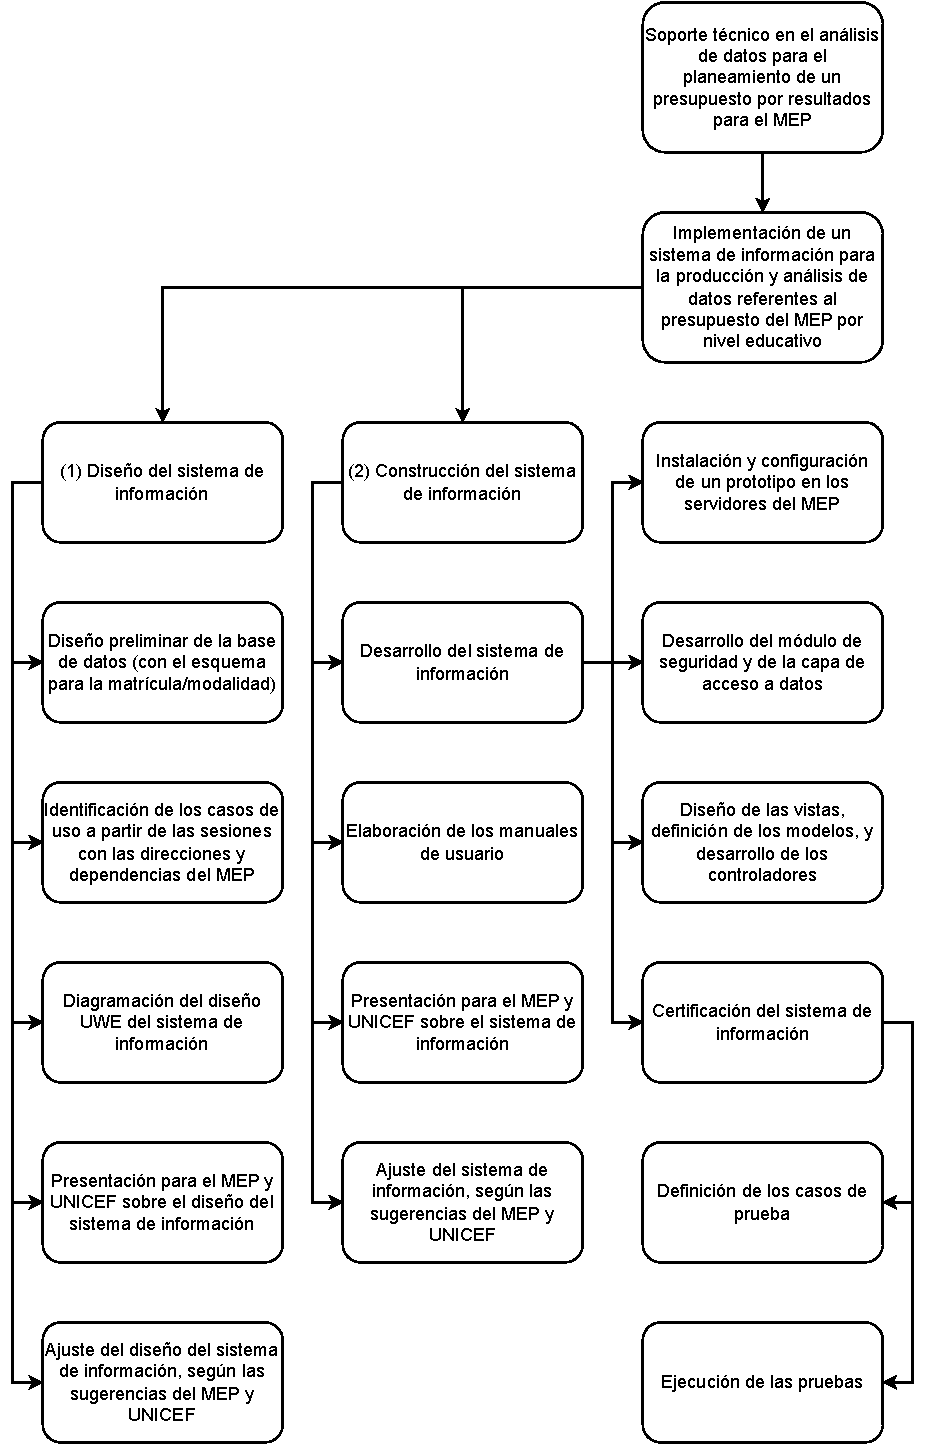
\includegraphics[width=320px, keepaspectratio=false]{edt1}
			\caption{Diagrama de la Estructura Desagregada de Trabajo, p\'agina 1.}
	\label{edt1}
\end{figure}

\begin{figure}
	\centering
		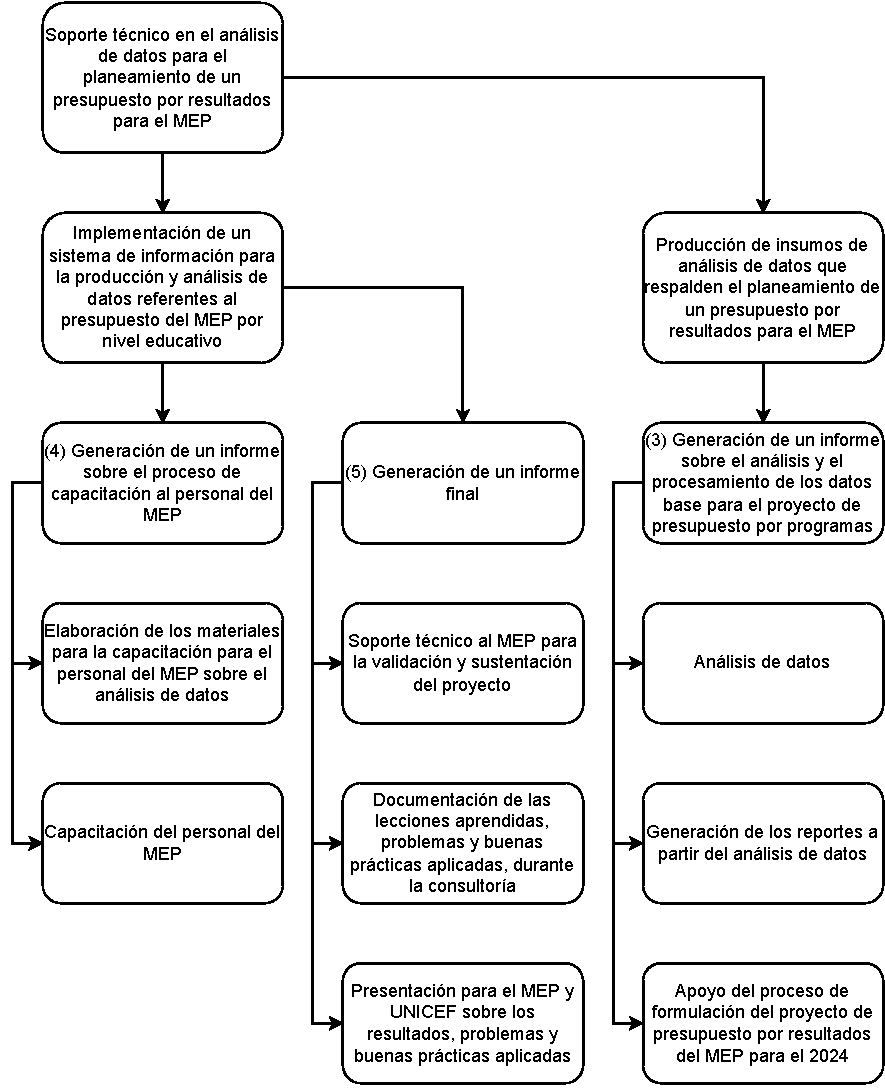
\includegraphics[width=320px, keepaspectratio=false]{edt2}
			\caption{Diagrama de la Estructura Desagregada de Trabajo, p\'agina 2.}
	\label{edt2}
\end{figure}

% --------------------------------------------------------------------------------------------------------------------------------
\section{Metodolog\'ia} \label{sec:methodology}

El proyecto de presupuesto por resultados consiste en un an\'alisis de datos que servir\'a como base para el planeamiento del presupuesto, y en el desarrollo de un sistema de informaci\'on que permita recopilar los conjuntos de datos necesarios para el an\'alisis \cite{trd}. Para desarrollar el sistema de informaci\'on ser\'a necesario identificar los casos de uso a partir de las sesiones con las direcciones y dependencias del ministerio.

El lenguaje formal que vamos a utilizar est\'a inspirado en el lenguaje Z\footnote{Un lenguaje para especificaciones, refinamientos y demostraciones.}, un lenguaje utilizado en las especificaciones de sistemas de informaci\'on, y el lenguaje gr\'afico que vamos a utilizar es el lenguaje \emph{UML-based Web Engineering} (UWE), un lenguaje basado en UML para el trabajo en la ingenier\'ia de aplicaciones Web.

El paradigma mediante el que vamos a elaborar el dise\~no del sistema de informaci\'on es el paradigma Programaci\'on Orientada a Objetos\footnote{En otras palabras, el dise\~no estar\'a basado en las interacciones entre los objetos que identifiquemos, interacciones de herencia, cohesi\'on, abstracci\'on, polimorfismo, acoplamiento y encapsulamiento.} (OOP por sus siglas en ingl\'es). El sistema implementar\'a el patr\'on de dise\~no Modelo Vista Controlador (MVC por sus siglas en ingl\'es), un patr\'on ampliamente utilizado en la ingenier\'ia de aplicaciones Web, debido a la notable adaptabilidad del patr\'on con la arquitectura de la Web.

El patr\'on Modelo Vista Controlador permite desarrollar cualquier aplicaci\'on Web en estructuras de datos, interfaces de usuario, y componentes log\'isticos; modelos, vistas y controladores respectivamente. En las aplicaciones Web que implementan este patr\'on, con frecuencia las vistas contienen el c\'odigo HTML, los modelos definen las estructuras de datos, y los controladoes implementan la log\'istica mediante la que se resuelve las peticiones provenientes del navegador.

\begin{figure}[H]
	\centering
		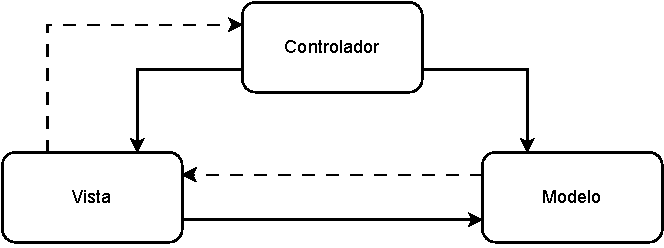
\includegraphics[width=240px, keepaspectratio=false]{mvc}
			\caption{Interacciones entre el modelo, la vista y el controlador.}
	\label{mvc}
\end{figure}

MySQL es un motor de bases de datos relacionales, multihilo y multiusuario, el m\'as utilizado en Internet, este es el motor que hemos propuesto para el sistema de informaci\'on. En caso de utilizar este motor, la base de datos podr\'a ser administrada mediante la aplicaci\'on MySQL-Workbench. La tecnolog\'ia que proponemos utilizar en el servidor Web es PHP mediante el \emph{framework} Phalcon. En caso de utilizar esta tecnolog\'ia, el sistema de informaci\'on podr\'ia ser desarrollado en el IDE Visual Studio Code.

% --------------------------------------------------------------------------------------------------------------------------------
\subsection{Identificaci\'on de las variables y entregables por objetivo espec\'ifico}

La siguiente es la lista de objetivos espec\'ificos en la secci\'on \ref{sec:subgoals}, a cada objetivo le siguen las variables y los entregables que le corresponden.

\begin{enumerate}
	\item Implementar una herramienta o sistema de informaci\'on para la producci\'on y an\'alisis de datos referentes al presupuesto del MEP por nivel educativo (preescolar, primaria y secundaria) \cite{trd}.
	
	\paragraph{Variables.}

	(1) Procesamiento actual de la informaci\'on necesaria para el planeamiento del presupuesto del ministerio, (2) Valoraci\'on por parte del ministerio y de UNICEF a cerca del dise\~no del sistema de informaci\'on, (3) Valoraci\'on por parte del ministerio y de UNICEF a cerca del sistema de informaci\'on, (4) Problemas durante las fases de dise\~no, construcci\'on, capacitaci\'on y soporte
	
	\paragraph{Entregables.}

	(a) Dise\~no del sistema de informaci\'on, (b) Desarrollo del sistema de informaci\'on, (c) Informe sobre el proceso de capacitaci\'on al personal del ministerio, (d) Informe final

	\item Producir insumos de an\'alisis de datos que respalden el planeamiento de un presupuesto por resultados para el Ministerio de Educaci\'on P\'ublica MEP para el a\~no 2024 \cite{trd}.
	
	\paragraph{Variables.}

	(5) Problemas durante la fase de an\'alisis de datos
	
	\paragraph{Entregables.}

	Informe sobre el an\'alisis y el procesamiento de los datos base para el proyecto de presupuesto por programas
\end{enumerate}

% --------------------------------------------------------------------------------------------------------------------------------
\subsection{Identificaci\'on de los atributos de cada variable}

El cuadro \ref{attrs} contiene, para cada variable identificada en la secci\'on \ref{sec:subgoals}, una definici\'on operacional y una definici\'on instrumental, i.e., una actividad y un recurso respectivamente, mediante los que sea posible satisfacer la variable.

\begin{table}[H]
	\centering
	\caption{Atributos para cada variable. Sobre la definici\'on operacional de la primera variable, seg\'un el Viceministro de Planificaci\'on Institucional y Coordinaci\'on Regional del MEP, ser\'an necesarias al menos una sesi\'on con Plataforma Saber, otra con Caricaco y otra con Estad\'istica.}
	\label{attrs}
	\begin{tabular}{p{0.1\linewidth}p{0.4\linewidth}p{0.4\linewidth}}
		\rowcolor[HTML]{FFFFFF}
		{\color[HTML]{000000} Variable} & {\color[HTML]{000000} Definici\'on operacional}                                           & {\color[HTML]{000000} Definici\'on instrumental} \\
		\hline
		1                               & Sesiones con las direcciones y dependencias del ministerio                                & Registro del audio de las sesiones \\
		2                               & Presentaci\'on para el ministerio y UNICEF sobre el dise\~no del sistema de informaci\'on & Registro del audio de la presentaci\'on \\
		3                               & Presentaci\'on para el ministerio y UNICEF sobre el sistema de informaci\'on              & Registro del audio de la presentaci\'on \\
		4                               & Atenci\'on de problemas                                                                   & Bitacorizaci\'on de cada problema y lecci\'on aprendida \\
		5                               & Atenci\'on de problemas                                                                   & Bitacorizaci\'on de cada problema y lecci\'on aprendida \\
	\end{tabular}
\end{table}

% --------------------------------------------------------------------------------------------------------------------------------
\section{Productos}

La lista a continuaci\'on describe a cada producto. El desarrollo de cada uno de estos productos, en conjunto, permite alcanzar el objetivo general planteado en la secci\'on \ref{sec:goal}. El primer producto corresponde a este documento.

\begin{enumerate}
	\item Propuesta de trabajo para el procesamiento y an\'alisis de datos referentes al presupuesto del MEP por nivel educativo (preescolar, primaria y
	secundaria) \cite{trd}
	\item Propuesta de dise\~no de una herramienta o sistema de informaci\'on para la producci\'on y an\'alisis de datos referentes al presupuesto del MEP por nivel
	educativo \cite{trd}
	\item Herramienta o sistema de informaci\'on para la producci\'on y an\'alisis de datos referentes al presupuesto del MEP por nivel educativo \cite{trd}
	\item Informe de an\'alisis y procesamiento de datos base para el proyecto de presupuesto por programas MEP 2024 \cite{trd}
	\item Informe sobre proceso de capacitaci\'on a personal del MEP \cite{trd}
	\item Informe final \cite{trd}
\end{enumerate}

% --------------------------------------------------------------------------------------------------------------------------------
\section{Insumos necesarios}

La siguiente es la lista de insumos necesarios para iniciar el desarrollo del sistema de informaci\'on. Los insumos est\'an agrupados seg\'un el producto para el que se requieren por primera vez.

\begin{itemize}
	\item (1) Lista de perfiles de usuario, en funci\'on de sus interacciones con el sistema de informaci\'on
	\item (2) Cat\'alogo de provincias, cantones y distritos, (3) \'Indice de desarrollo social seg\'un la regi\'on de planificaci\'on, (4) Nomenclatura para la identificaci\'on de localidades, (5) Formato de la n\'omina de centros educativos, (6) Documentaci\'on de los procesos que requieran automatizaci\'on, (7) Sujerencias del ministerio a cerca del dise\~no

	\item (8) Datos de acceso a los servidores del ministerio, (9) Sujerencias del ministerio a cerca del sistema de informaci\'on
	\item (10) Datos de acceso a la base de datos de Territorium, (11) F\'ormulas del c\'alculo actual del presupuesto del ministerio, (12) Formato del reporte de transporte, (13) Formato del reporte de alimentos, (14) Especificaciones a cerca del tablero del sistema de informaci\'on
\end{itemize}

% --------------------------------------------------------------------------------------------------------------------------------
\section{Actores que deben vincularse en las acciones} \label{sec:prof}

La siguiente es la lista preliminar de perfiles de usuario del sistema de informaci\'on. La lista fue proveida por el Viceministro de Planificaci\'on Institucional y Coordinaci\'on Regional del MEP.

\begin{enumerate}
	\item \emph{Direcci\'on de Planificaci\'on}. Los funcionarios del ministerio encargados de la planificaci\'on, monitoreo y evaluaci\'on del sistema educativo. Estos actores, mediante el sistema de informaci\'on, podr\'an acceder a datos actualizados, analizar indicadores y tomar decisiones informadas en pol\'iticas educativas y programas.

	\item \emph{Direcciones Generales o Departamentos del Ministerio de Educaci\'on}. Los directores y funcionarios de las diferentes direcciones generales o departamentos del ministerio, como la direcci\'on de RR HH, el departamento de curr\'iculo, el departamento de evaluaci\'on, el departamento de comedores y transporte, entre otros. Estos actores, mediante el sistema de informaci\'on, podr\'an acceder a datos espec\'ificos relacionados con sus \'areas de responsabilidad para apoyar la toma de decisiones.

	\item \emph{Instituciones Educativas (desde preescolar hasta secundaria)}. Los directores, docentes y personal administrativo de las instituciones educativas. Estos actores, mediante el sistema de informaci\'on, podr\'an registrar y acceder a datos de los estudiantes, el personal docente, los planes de estudio, la asistencia, las calificaciones y otra informaci\'on relevante para la gesti\'on educativa.

	\item \emph{Estudiantes}. Los estudiantes y sus padres o tutores. Estos actores, mediante el sistema de informaci\'on, podr\'an acceder a ciertos m\'odulos para consultar su progreso acad\'emico, registrar su asistencia, acceder a recursos educativos en l\'inea y participar en actividades relacionadas con el aprendizaje.

	\item \emph{Personal de apoyo educativo}. Los profesionales encargados de brindar apoyo educativo, como psic\'ologos, orientadores, terapeutas, entre otros. Estos actores, mediante el sistema de informaci\'on, podr\'an registrar y acceder a datos de los estudiantes que requieran atenci\'on especial, y podr\'an planificar y monitorear intervenciones y programas de apoyo.

	\item \emph{Funcionarios de control y evaluaci\'on}. Los auditores, inspectores u otros funcionarios encargados de evaluar la calidad y eficiencia del sistema educativo. Estos actores, mediante el sistema de informaci\'on, podr\'an obtener datos relevantes, realizar seguimiento y evaluaci\'on de indicadores, y generar informes de control y rendici\'on de cuentas.

	\item \emph{Proveedores de servicios educativos}. Los proveedores externos de servicios educativos, como editores de libros de texto, proveedores de plataformas de aprendizaje en l\'inea, entre otros. Estos actores, mediante el sistema de informaci\'on, podr\'an interactuar con el sistema de informaci\'on para suministrar recursos y servicios educativos.

	\item \emph{Equipo t\'ecnico}. Los profesionales encargados del mantenimiento, actualizaci\'on y desarrollo tecnol\'ogico, profesionales como desarrolladores, administradores de bases de datos, personal de soporte t\'ecnico, entre otros.

	\item \emph{Consultores}. Consultores externos contratados para brindar asesor\'ia y soporte en la implementaci\'on y optimizaci\'on del sistema de informaci\'on, o contratados para proporcionar recomendaciones y asistencia t\'ecnica.

	\item \emph{Padres de familia o tutores}. Los padres de familia o tutores de los estudiantes. Estos actores, mediante el sistema de informaci\'on, podr\'an acceder a informaci\'on sobre el progreso acad\'emico de sus hijos, informaci\'on sobre calificaciones, asistencia, y otros datos relevantes. El sistema tambi\'en les facilitar\'a la comunicaci\'on con las instituciones educativas.

	\item \emph{Personal de gesti\'on financiera}. Los funcionarios encargados de la gesti\'on financiera del ministerio, como los responsables de presupuesto y finanzas. Estos actores, mediante el sistema de informaci\'on, podr\'an acceder a datos financieros, realizar\'a seguimiento de los gastos y financiamiento de programas educativos, y generar informes financieros.

	\item \emph{Organismos externos}. Organismos gubernamentales, organizaciones no gubernamentales, agencias de cooperaci\'on internacional u otros actores externos que trabajen en colaboraci\'on con el ministerio. Estos actores, mediante el sistema de informaci\'on, podr\'an acceder a datos relevantes y colaborar en la toma de decisiones y evaluaci\'on de programas educativos.

	\item \emph{Personal de capacitaci\'on y desarrollo profesional}. Los responsables de la capacitaci\'on y desarrollo profesional del personal docente y administrativo. Estos actores, mediante el sistema de informaci\'on, podr\'an planificar, gestionar y evaluar programas de formaci\'on y desarrollo profesional del personal educativo.

	\item \emph{Medios de comunicaci\'on}. Los representantes de medios de comunicaci\'on, como periodistas y reporteros. Estos actores, mediante el sistema de informaci\'on, podr\'an obtener datos y generar reportajes o noticias relacionadas con el sistema educativo y las pol\'iticas educativas.

	\item \emph{Usuarios externos interesados}. Cualquier interesado en la informaci\'on del sistema educativo, investigadores, acad\'emicos, y ciudadanos en general. Estos actores, mediante el sistema de informaci\'on, podr\'an acceder a ciertos datos para realizar investigaciones, an\'alisis o seguimiento de indicadores educativos.
\end{enumerate}

% --------------------------------------------------------------------------------------------------------------------------------
\section{Cronograma de actividades} \label{sec:crono}

La siguiente es la lista de actividades mediante las que los productos ser\'an desarrollados. Cada actividad est\'a indexada mediante una fecha de finalizaci\'on, una fecha determinada a partir de la fecha de entrega del producto correspondiente, seg\'un el documento ``T\'erminos de referencia para contrataci\'on de consultor(a)/contratista individual'', el documento que contiene la fecha de entrega de cada producto \cite{trd}.

\begin{tasks}[](2)
	\task[]
	\begin{description}
		\item[2023\,04\,20] Identificaci\'on de los casos de uso a partir de las sesiones con las direcciones y dependencias del MEP
		\item[2023\,04\,28] Dise\~no preliminar de la base de datos
		\item[2023\,05\,02] Diagramaci\'on del dise\~no UWE del sistema de informaci\'on
		\item[2023\,05\,04] Presentaci\'on para el MEP y UNICEF sobre el dise\~no del sistema de informaci\'on
		\item[2023\,05\,11] Ajuste del dise\~no del sistema de informaci\'on, seg\'un las sugerencias del MEP y UNICEF
	\end{description}
	\task[]
	\begin{description}
		\item[2023\,05\,15] Instalaci\'on y configuraci\'on de un prototipo en los servidores del MEP
		\item[2023\,05\,19] Definici\'on del espacio de trabajo
		\item[2023\,05\,26] Desarrollo del m\'odulo de seguridad y de la capa de acceso a datos
		\item[2023\,06\,02] Dise\~no de las vistas, definici\'on de los modelos, y desarrollo de los controladores
		\item[2023\,06\,05] Definici\'on de los casos de prueba
		\item[2023\,06\,06] Ejecuci\'on de las pruebas
		\item[2023\,06\,07] Elaboraci\'on de los manuales de usuario
		\item[2023\,06\,09] Presentaci\'on para el MEP y UNICEF sobre el sistema de informaci\'on
		\item[2023\,06\,15] Ajuste del sistema de informaci\'on, seg\'un las sugerencias del MEP y UNICEF
	\end{description}
	\task[]
	\begin{description}
		\item[2023\,07\,06] An\'alisis de datos
		\item[2023\,07\,13] Generaci\'on de los reportes a partir del an\'alisis de datos
		\item[2023\,07\,20] Apoyo del proceso de formulaci\'on del proyecto de presupuesto por resultados del MEP para el 2024
	\end{description}
	\task[]
	\begin{description}
		\item[2023\,08\,10] Elaboraci\'on de los materiales para la capacitaci\'on para el personal del MEP sobre el an\'alisis de datos
		\item[2023\,08\,17] Capacitaci\'on del personal del MEP
	\end{description}
	\task[]
	\begin{description}
		\item[2023\,08\,31] Soporte t\'ecnico al MEP para la validaci\'on y sustentaci\'on del proyecto
		\item[2023\,09\,07] Documentaci\'on de las lecciones aprendidas, problemas y buenas pr\'acticas aplicadas, durante la consultor\'ia
		\item[2023\,09\,14] Presentaci\'on para el MEP y UNICEF sobre los resultados, problemas y buenas pr\'acticas aplicadas
	\end{description}
\end{tasks}

% --------------------------------------------------------------------------------------------------------------------------------
\section{Conclusiones y recomendaciones}

Seg\'un el cronograma en la secci\'on \ref{sec:crono}, el tiempo disponible para realizar las tareas de desarrollo (del m\'odulo de seguridad, de la capa de acceso a datos, de las vistas, los modelos y los controladores), control de calidad, y elaboraci\'on de manuales y presentaci\'ones, es de dos semanas. Sin embargo, el desarrollo de los casos de uso inferibles de la lista en la secci\'on \ref{sec:prof} puede requerir m\'as de dos semanas de tiempo, por lo que puede ser recomendable seleccionar para desarrollar los casos de uso indispensables para la producci\'on y an\'alisis de datos referentes al presupuesto del ministerio para el a\~no 2024, el objetivo general del proyecto, planteado en la secci\'on \ref{sec:goal}, y dejar para una segunda fase, el desarrollo de los dem\'as casos de uso.

% --------------------------------------------------------------------------------------------------------------------------------
\bibliographystyle{IEEEtran}
\bibliography{refs}

% --------------------------------------------------------------------------------------------------------------------------------
\section{Sem\'antica}

\begin{table}[H]
	\centering
	\caption{Sem\'antica}
	%\label{semantics}
	\begin{tabular}{p{0.25\linewidth}p{0.7\linewidth}}
		%\rowcolor[HTML]{FFFFFF}
		%{\color[HTML]{000000} S\'imbolo} & {\color[HTML]{000000} Definici\'on} \\
		\hdashline%\rowcolor{black!5}
		Caso de prueba & Escenario en el que se requiere verificar un comportamiento del sistema de informaci\'on. \\
		\hdashline%\rowcolor{black!5}
		Caso de uso & Descripci\'on de la forma en que un usuario interactua con un sistema de informaci\'on para realizar una tarea. \\
		\hdashline%\rowcolor{black!5}
		EDT & Estructura de Descomposici\'on del Trabajo, conocida en ingl\'es como \emph{Work Breakdown Structure} o WBS, en el contexto de la gesti\'on de proyectos se le considera una descomposici\'on jer\'arquica orientada al entregable, del trabajo a ser ejecutado por el equipo de proyecto. \\
		\hdashline%\rowcolor{black!10}
		HTML & Lenguaje de marcado hipertextual, o en ingl\'es, \emph{Hypertext Markup Language}, es mediante el que se configura la ret\'icula y el contenido de las p\'aginas Web. \\
		\hdashline%\rowcolor{black!5}
		IDE & Entorno de desarrollo integrado, o en ingl\'es \emph{Integrated Development Environment}, relativo a editores de texto plano que facilitan la escritura de c\'odigo en alg\'un lenguaje de programaci\'on. \\
		\hdashline%\rowcolor{black!10}
		Inferface & Conexi\'on f\'isica y funcional entre dos mecanismos de cualquier tipo que permite la comunicaci\'on entre tales mecanismos. \\
		\hdashline%\rowcolor{black!10}
		MVC & Patr\'on de arquitectura de software que separa los datos y la l\'ogica de negocio de la interface de usuario y el m\'odulo encargado de gestionar los eventos y las comunicaciones. \\
		\hdashline%\rowcolor{black!10}
		MySQL & Motor de bases de datos relacionales, multihilo y multiusuario. \\
		\hdashline%\rowcolor{black!10}
		MySQL Workbench & Aplicaci\'on que facilita la administraci\'on de las bases de datos MySQL. \\
		\hdashline%\rowcolor{black!10}
		Phalcon & \emph{Framework} para el desarrollo de aplicaciones Web con PHP, desarrollado en el lenguaje C. \\
		\hdashline%\rowcolor{black!10}
		Prototipo & Versi\'on preliminar de un sistema de informaci\'on. \\
		\hdashline%\rowcolor{black!10}
		Territorium & Empresa encargada de la carga en tiempo real de datos geolocalizados para el MEP. \\
		\hdashline%\rowcolor{black!10}
		UML & Lenguaje Unificado de Modelado, o en ingl\'es \emph{Unified Modeling Language}, es un lenguaje gr\'afico para el modelado de sistemas de informaci\'on. Se utiliza en especificaciones, en documentaciones en general. \\
		\hdashline%\rowcolor{black!10}
		UWE & En ingl\'es \emph{UML-Based Web Engineering}, es un lenguaje gr\'afico para el modelado de sistemas de informaci\'on Web, es una extensi\'on del UML. \\
		\hdashline%\rowcolor{black!10}
		Visual Studio Code & Entorno de desarrollo integrado de software libre, desarrollado por Microsoft, provee soporte para lenguajes como SQL, C\#, Java, PHP, JavaScript, CSS y HTML. Puede ser extendido mediante complementos. \\
		\hdashline%\rowcolor{black!10}
		Z & Lenguaje formal utilizado en las especificaciones de sistemas de informaci\'on, facilita el refinamiento de las especificaciones y el desarrollo de las demostraciones.
	\end{tabular}
\end{table}

% --------------------------------------------------------------------------------------------------------------------------------
\end{document}
